\chapter{Basic Notions} 

To make this work more self-contained, we briefly introduce basic notions and concepts used in the later chapters. 
Details can be found in \todo{doplnit odkazy na nejaka skripta, klidne nekolik; jednim z nich by mel byt Hartley, Zisserman: Multiple View Geometry}.
% TODO v tehle sekci ale chceme rozebirat jen matematicke a image processing pojmy, ne ty softwarove, coz je otazka, jestli bychom to nemeli nejak zminit... ale mozna ani ne... nevim

\begin{framed} 
% TODO 
\todo{Co budeme potrebovat zavest:} 
\begin{itemize} 
\item convolution 
\item image derivatives 
\item gaussian image derivatives 
\item sum of absolute differences 
\item entropy, mutual information 
\item hessian, laplacian 
\item homogeneous coordinates 
\item camera model (mozna do sekce o MVG?) 
\item fundamental matrix (mozna do sekce o MVG?) 
\end{itemize} 
\end{framed} 

\section{Hessian matrix}

% feature detectors and interest points descriptors employ the Hessian matrix of the image.
The Hessian matrix describes a second-order behavior of a function around a particular point. 

\begin{definition} 
\term{The Hessian matrix of a function $f: \Rn \to \R$ at $\x \in \Rn$} is a matrix $H_f(\x)$ of the second order partial derivatives of $f$ evaluated at $\x$: %~=~(x_1, \ldots, x_n)$: 
\begin{align*} 
H_f(\x) := 
\begin{pmatrix} 
\fpp{ \partial x_1^2 }              &   \fpp{ \partial x_1 \partial x_2 }   &   \ldots   &   \fpp{ \partial x_1 \partial x_n }   \\ 
\fpp{ \partial x_2 \partial x_1 }   &   \fpp{ \partial x_2^2 }              &   \ldots   &   \fpp{ \partial x_2 \partial x_n }   \\ 
\hdotsfor[2]{4} \\ 
\fpp{ \partial x_n \partial x_1 }   &   \fpp{ \partial x_n \partial x_2 }   &   \ldots   &   \fpp{ \partial x_n^2 }  
\end{pmatrix}. 
\end{align*} 
If any of the partial derivatives on the right-hand side are undefined, we say that the Hessian matrix is also undefined.
% \[ H(f, \x) = \left(\begin{array}{c}  
% \frac{\partial^2 f}{\partial x_1^2} \frac{\partial^2 f}{\partial x_1 \partial x_2} 
% \cdots \frac{\partial^2 f}{\partial x_1 \partial x_n}\\
% \frac{\partial^2 f}{\partial x_2 \partial x_1} \frac{\partial^2 f}{\partial x_2^2} 
% \cdots \frac{\partial^2 f}{\partial x_2\partial x_n}\\
% \cdots \cdots \cdots \\
% \frac{\partial^2 f}{\partial x_n \partial x_1} \frac{\partial^2 f}{\partial x_n \partial x_2} 
% \cdots \frac{\partial^2 f}{\partial x_n^2}
% 
% \end{array}\right)  \]
\end{definition} 
Within the context of image processing, the function $f$ typically corresponds to the input image and derivatives are replaced either by differences between the intensity levels of neighbouring pixels or Gaussian derivatives. 

The Hessian matrix forms a basis for a basic feature detector (called Hessian detector), which selects the image positions $\x$ locally maximizing $\det(H(I, \x)),$ where $I$ is the input image.
This leads to a detection of corners and features forming highly textured areas of size roughly comparable to the variance of the Gaussian kernel used to compute the Gaussian derivatives. % TODO zkontrolovat, jestli to neni nesmysl

\section{Integral images}

% Later in this work we work with the term of integral images. 
\term{An integral image}, also known as \term{summed area table}, allows fast and efficient computation of a sum of image intesity values inside an arbitrary rectangular area.
A pixel of an integral image represents the sum of all of the original image's pixels that lie to the left and above the considered position: 
\begin{equation*}
\K_I(\x) := \sum_{i \le x} \sum_{j \le y} I(i,j),
\end{equation*}
where $\K$ is the resulting integral image, \emph{I} is the input image image, and $\x = \vect{(x, y)}^{T}$ is a location of a pixel.

An advantage of the integral image is that we are able to compute it using only one pass through the original image. 
Moreover, once we have calculated the integral image, only three integer operations and four memory accesses are required to calculate the sum 
of the original intensities inside any rectangular region (see Figure \ref{fig:integral}).

\begin{figure}[h]
  \centering{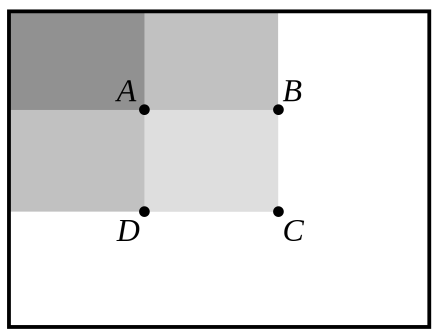
\includegraphics[width=96mm]{img/integral_image.png}}
  \caption{The sum of any rectangular region can be calculated by only three additions. \todo{napsat konkretni vzorec}}
  \label{fig:integral}
\end{figure}
